\documentclass[11pt]{article}

\usepackage{centernot}
\usepackage{amssymb}
\usepackage{xcolor}
\definecolor{myblue}{RGB}{0, 0, 255} 
\definecolor{mygreen}{RGB}{0, 180, 80}
\definecolor{myred}{RGB}{153, 0, 0}
\definecolor{myorange}{RGB}{255, 153, 51}
\definecolor{mypurple}{RGB}{102, 0, 204}
\usepackage{verbatim}
\usepackage{multicol}
\usepackage{enumitem}
\usepackage{amsfonts}
\usepackage{amsmath}
\usepackage[utf8]{inputenc}
\usepackage[export]{adjustbox}  % for correct logo rendering
\usepackage{fancyhdr}  % for header/footer formatting
\usepackage{hyperref}  % for hyper-references
\usepackage{datetime}  % to update month in footer
\usepackage{array}  % more flexible tables
\usepackage[includeheadfoot,
            left=1in,
            right=1in,
            top=0.75in,
            bottom=0.75in,
            headheight=40pt]{geometry} % geometry needs to know headheight to correctly render the footer
\usepackage{tikz} % For drawing grid boxes

\definecolor{darkblue}{RGB}{0, 0, 139}
\definecolor{lightblue}{RGB}{173, 216, 230}

% desired format for footer
\newdateformat{monthyeardate}{%
  \monthname[\THEMONTH] \THEYEAR}

% set up header/footer
\pagestyle{fancy}
\fancyhf{}  % clear all headers/footers
\renewcommand{\headrulewidth}{0pt}  % remove header rule
\renewcommand{\footrulewidth}{0pt}  % remove footer rule

% set up header

\fancypagestyle{firstpage}{
    \fancyhead[L]{
    \vspace{0pt}
    \hspace{-8pt}
    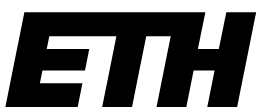
\includegraphics[width=0.1\textwidth]{docimgs/eth_logo_kurz_pos.png}\\
    \textbf{Swiss Federal Institute of Technology}\\
    \textbf{Zurich}\\
    %\textbf{ } \\
    
    }    

    \fancyhead[R]{
    \raggedleft
    %\vspace{20pt}
    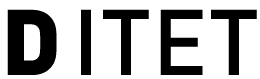
\includegraphics[width=0.13\textwidth]{docimgs/eth_ditet_logo_pos.png}\\
     \textbf{Dept. of Information Technology and} \\ \textbf{Electrical Engineering}  \\
     %\textbf{Chair for Mathematical Information} \\ \textbf{Information Science} \\

    }
}

% set up footer
\fancyfoot[L]{mdietz, ÜS 6}
\fancyfoot[C]{\thepage}
\fancyfoot[R]{\monthyeardate\today}

% set up section/subsection titles
\renewcommand{\thesection}{\arabic{section}}
\renewcommand{\thesubsection}{\arabic{subsection}}

% command used for simply emphasizing suggestions
\newcommand{\suggestion}[1]{{\itshape #1}}

%--- commands for transform arrows----------------
\newcommand{\transform}[2]{%
    \begin{tikzpicture}
        % Open circle
        \draw[thick] (0,0) circle (0.1);
        % Line with number above and adjustable length
        \draw[thick] (0.1,0) -- (#2,0) node[midway, above] {#1};
        % Filled circle
        \filldraw[thick] (#2,0) circle (0.1);
    \end{tikzpicture}%
}
\newcommand{\invtransform}[2]{%
    \begin{tikzpicture}
        % filled circle
        \filldraw[thick] (0,0) circle (0.1);
        % Line with number above and adjustable length
        \draw[thick] (0.1,0) -- (#2 -0.1,0) node[midway, above] {#1};
        % open circle
        \draw[thick] (#2,0) circle (0.1);
    \end{tikzpicture}%
}
\newcommand{\verticaltransform}[4]{%
    \begin{tikzpicture}
        % Open circle at the bottom with text below
        \filldraw[thick] (0,0) circle (0.1) node[below=3pt] {$#4$};
        % Vertical line with number on the left
        \draw[thick] (0,0.1) -- (0,#2 -0.1) node[midway, left] {#1};
        % Filled circle at the top with text above
        \draw[thick] (0,#2) circle (0.1) node[above=3pt] {$#3$};
    \end{tikzpicture}%
}
\newcommand{\verticalinvtransform}[4]{%
    \begin{tikzpicture}
        % Open circle at the bottom with text below
        \draw[thick] (0,0) circle (0.1) node[below=3pt] {$#4$};
        % Vertical line with number on the left
        \draw[thick] (0,0.1) -- (0,#2) node[midway, left] {#1};
        % Filled circle at the top with text above
        \filldraw[thick] (0,#2) circle (0.1) node[above=3pt] {$#3$};
    \end{tikzpicture}%
}

\begin{document}
\thispagestyle{firstpage}

\setlength{\headheight}{1 \baselineskip}  % accomodate header
\setlength{\parindent}{0pt}  % remove initial paragraph indent
\setlength{\parskip}{\baselineskip}  % add skip between paragraphs

\vspace*{-5px}
\section*{Übungsstunde 6}

\section*{Themenüberblick}
\begin{itemize}
    \item \textbf{Analoge Lineare Systeme im Frequenzbereich:}
    \item[] Kurze Repetition: Fouriertransformation und Eigenschaften
    \item[] Eigenfunktionen von LTI Systemen
    \item[] Antwort von LTI-Systemen im Frequenzbereich
    \item[] Kaskadierung von LTI-Systemen
    \item \textbf{Spezielle Eingangssignale von LTI-Systemen}
    \item[] Allgemeine Schwingungen
    \item[] Sinusförmige Eingangssignale 
    \item[] Einschaltvorgänge
    \item[] Periodische Eingangssignale und Fourierreihen
    \item[] Deltakamm und Poissonsche Summenformel
\end{itemize}

\section*{Aufgaben für diese Woche}
\vspace{-0.5cm}

Nochmals dieselben wie letzte Woche und \textbf{69}, \textbf{70}, \textbf{71}, \textbf{72}, 73, \textbf{74}\\
\vspace{-0.5cm}

Die \textbf{fettgedruckten} Übungen empfehle ich, weil sie wesentlich zu eurem Verständnis der Theorie beitragen und/oder sehr prüfungsrelevant sind.

\vfill \null
\pagebreak

\section*{Repetition: Eigenschaften der Fouriertransformation}
\vspace*{-0.5cm}
\subsection*{Definition}
\vspace*{-0.5cm}
\fcolorbox{darkblue}{lightblue}{%
\parbox{\dimexpr\linewidth-2\fboxsep-2\fboxrule\relax}{
    $$\text{(FT)} \hspace{20pt} \hat{x}(f) = (\mathcal{F}x)(f) = \int_{-\infty}^{\infty}x(t)e^{-2\pi i f t}\text{d}t$$
    $$\text{(IFT)} \hspace{10pt} x(t) = (\mathcal{F}^{-1}\hat{x})(t) = \int_{-\infty}^{\infty}\hat{x}(f)e^{2\pi i f t}\text{d}f$$
}}%

\vspace*{-0.5cm}
\subsection*{Riemann-Lebesgue Lemma}
\vspace*{-0.5cm}
Es sei $x$ ein absolut integrierbares Signal, d.h. $x \in L^1$. Dann ist $(\mathcal{F}x)(f) = \hat{x}(f)$ stetig und $\displaystyle\lim_{|f| \to \infty} \hat{x}(f) = 0$.

\subsection*{Formelsammlung}
\begin{center}
    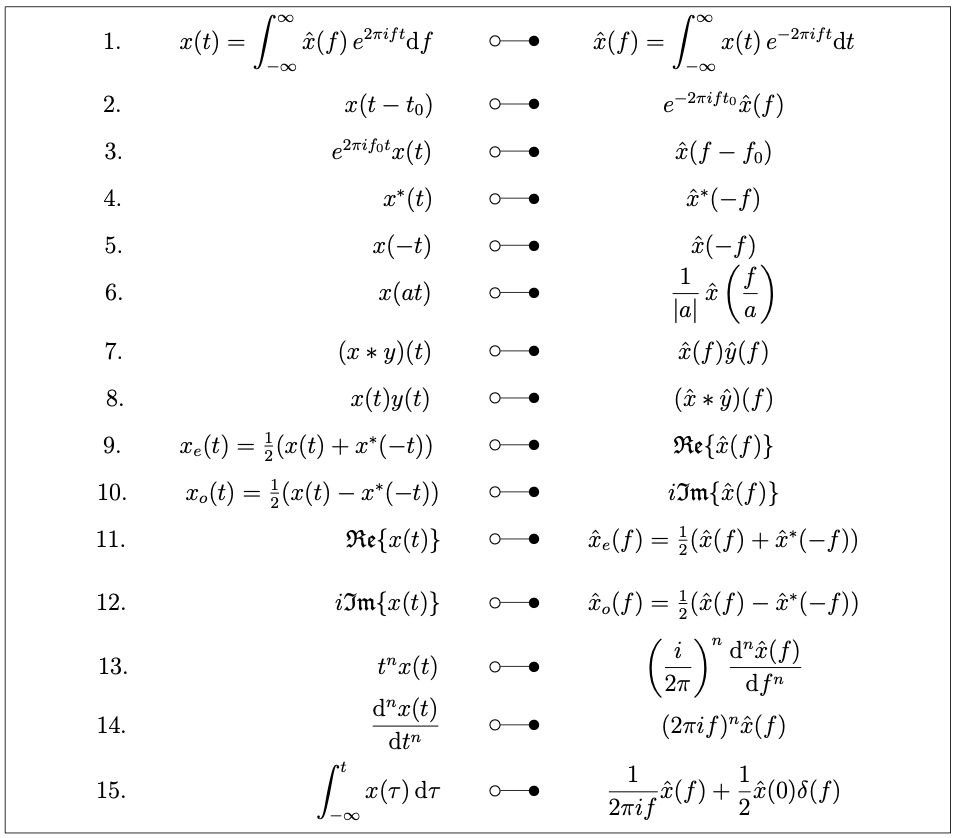
\includegraphics[width=0.8\linewidth]{docimgs/FT_eigenschaften.png}
\end{center}

\pagebreak

\subsection*{Repetition: Parseval und Plancherel}

\fcolorbox{darkblue}{lightblue}{%
    \parbox{\dimexpr\linewidth-2\fboxsep-2\fboxrule\relax}{
    \begin{center}
        \textbf{Plancherelsche Identität:}
    \end{center}
    $$\langle x, y \rangle = \int_{-\infty}^{\infty} x(t)y^\ast (t)\text{d}t = \int_{-\infty}^{\infty}\hat{x}(f)\hat{y}^\ast(f)\text{d}f = \langle \hat{x}, \hat{y} \rangle$$
    \begin{center}
        \textbf{Parsevalsche Beziehung:}
    \end{center}
    $$||x||^2 = \langle x, x \rangle = \int_{-\infty}^{\infty} |x(t)|^2\text{d}t = \int_{-\infty}^{\infty}|\hat{x}(f)|^2\text{d}f = \langle \hat{x}, \hat{x} \rangle = ||\hat{x}||^2$$
    }}

\subsection*{Aufgabe 66}
\vspace*{-0.5cm}
Von einem Signal $x(t)$ ist die Fouriertransformierte gegeben als 
$$\hat{x}(f) = \begin{cases}
    1, \hspace{15pt} |f| \leq f_0\\
    0, \hspace{15pt} |f| > f_0
\end{cases}$$
Berechnen Sie die Energie des Signals $y(t) = \displaystyle\frac{\text{d}^2x(t)}{\text{d}t^2}$ gegeben durch
$$E_y = \int_{-\infty}^\infty |y(t)|^2 \text{d}t$$


\begin{tikzpicture}
    % Define the box size and grid spacing
    \draw[step=0.5cm,gray!50,very thin] (0,0) grid (16.5,6.5
    ); % (0,0) is bottom-left corner, (10,10) is top-right corner
\end{tikzpicture}

\vfill \null
\pagebreak

\subsection*{Prüfungsaufgabe: Sommer 2019, Aufgabe 2}

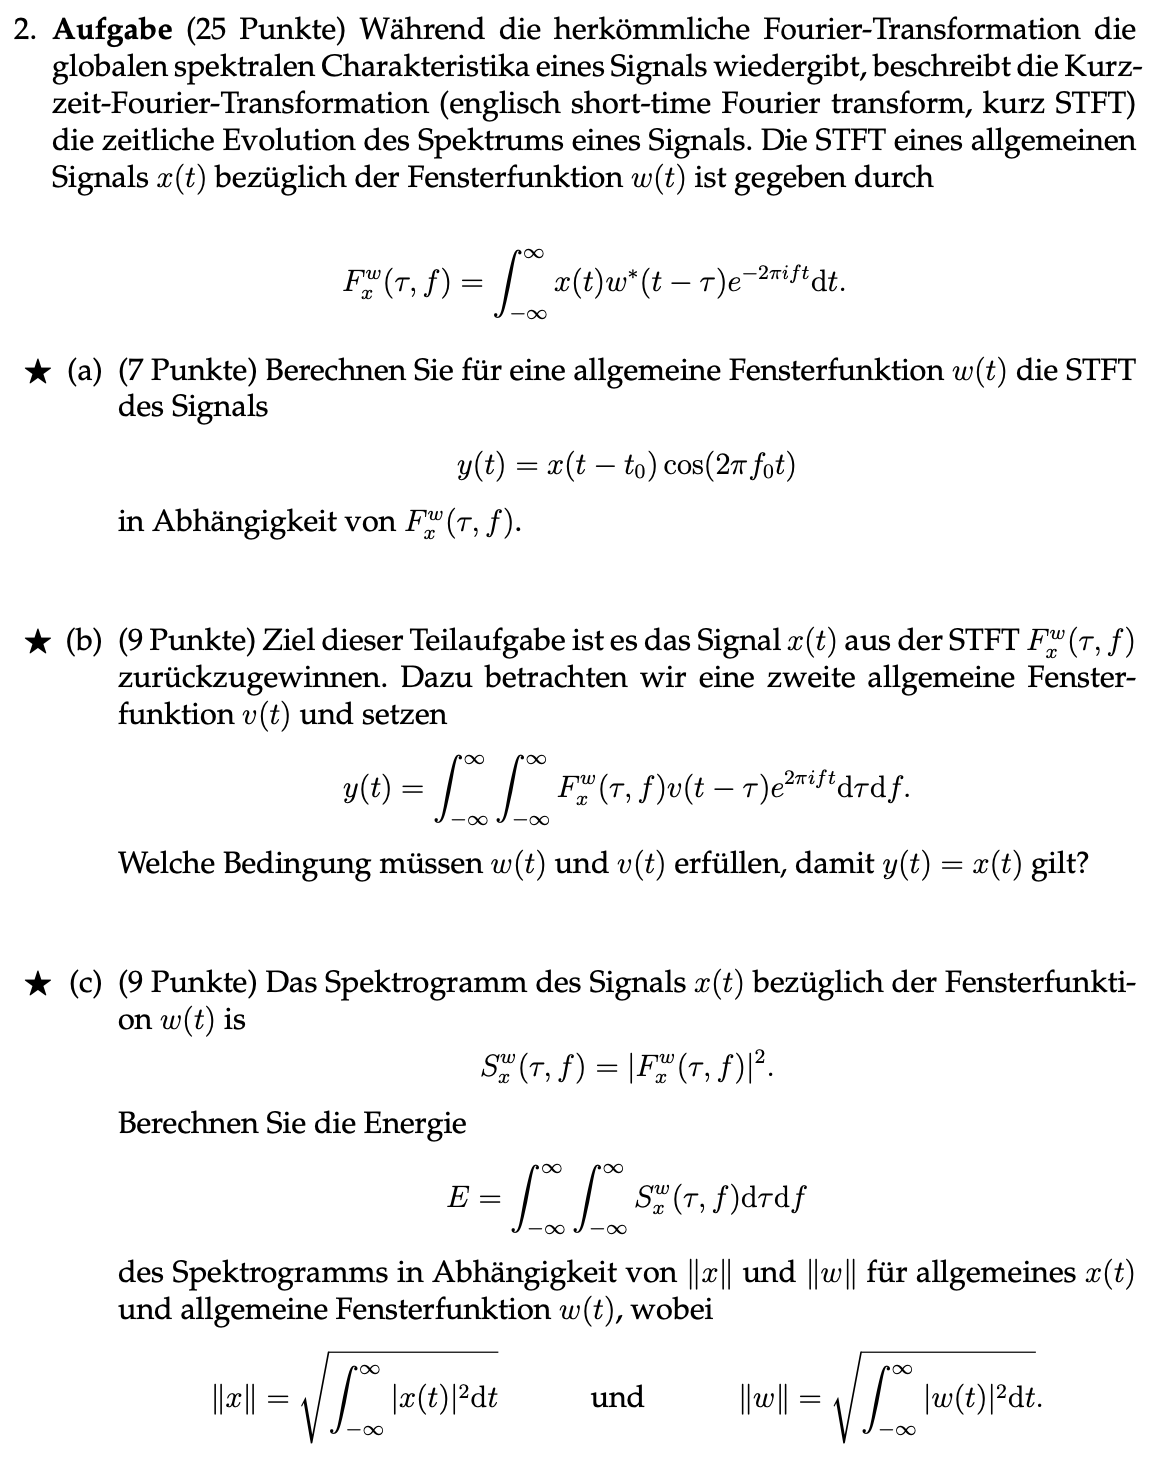
\includegraphics[width=0.9\linewidth]{docimgs/2019_ex2.png}


\vfill \null
\pagebreak


\begin{tikzpicture}
    % Define the box size and grid spacing
    \draw[step=0.5cm,gray!50,very thin] (0,0) grid (16.5,21
    ); % (0,0) is bottom-left corner, (10,10) is top-right corner
\end{tikzpicture}

\pagebreak


\begin{tikzpicture}
    % Define the box size and grid spacing
    \draw[step=0.5cm,gray!50,very thin] (0,0) grid (16.5,21
    ); % (0,0) is bottom-left corner, (10,10) is top-right corner
\end{tikzpicture}

\pagebreak

\section*{Eigenfunktionen analoger LTI-Systeme}
\vspace*{-0.5cm}
\begin{itemize}[leftmargin=0pt]
    \item[] \textbf{Reminder}: Eigenvektoren $x$ (z.B. Vektoren in $\mathbb{R}^n$) sind Vektoren, die die Gleichung $Hx = \lambda x$ erfüllen, wobei $H$ ein System (z.B. eine Matrix) ist. $\lambda$ nennt man den dazugehörigen Eigenwert.
    \item[] Wir wollen nun die Eigenfunktionen von analogen LTI Systemen finden. Das heisst, wir wollen $x(t)$ finden, sodass $y(t) = (Hx)(t) = \lambda x(t)$ gilt.
    \item[] \begin{center}
        
\includegraphics[width=0.9\linewidth]{docimgs/System_Blockschaltbild.png}
    \end{center}
    \item[] \textbf{Eingangssignal}: Wähle $x(t)= e^{2\pi i f_0 t}$ (komplexe Exponentialfunktion)
    \item[] Wir wenden nun darauf das LTI-System $H$ an:
    $$y(t) = (x \ast h)(t) = \int_{-\infty}^\infty x(t-\tau)h(\tau) \text{d}\tau = \int_{-\infty}^\infty e^{2 \pi i f_0 (t-\tau)} h(\tau) \text{d}\tau = e^{2 \pi i f_0 t} \underbrace{\int_{-\infty}^\infty h(\tau) e^{-2\pi i f_0 \tau} \text{d}\tau}_{\hat{h}(f_0)} $$
    $$\text{Es folgt: } \hspace{20pt} (He^{2 \pi i f_0 \cdot})(t) = \hat{h}(f_0)e^{2 \pi i f_0 t}$$
    \item[] \fcolorbox{darkblue}{lightblue}{\parbox{\dimexpr\linewidth-2\fboxsep-2\fboxrule\relax}{
    \textbf{Kunstgriff:}\\
    Die Funktionen $e^{2\pi i f_0 t}$ sind Eigenfunktionen von LTI-Systemen mit zugehörien Eigenwerten $\hat{h}(f_0)$
    }}%
\end{itemize}

\vspace*{-0.5cm}
\subsection*{Antwort von LTI-Systemen im Frequenzbereich}
\vspace*{-0.5cm}

\begin{tikzpicture}
    % Define the box size and grid spacing
    \draw[step=0.5cm,gray!50,very thin] (0,0) grid (16.5,7
    ); % (0,0) is bottom-left corner, (10,10) is top-right corner
\end{tikzpicture}

Somit gilt 
{\setlength{\fboxsep}{2pt} % Adjust padding for this box only
\fcolorbox{darkblue}{lightblue}{$\widehat{(x \ast h)}(f) = \hat{x}(f) \hat{h}(f)$} und in ähnlicher Weise {\setlength{\fboxsep}{2pt} % Adjust padding for this box only
\fcolorbox{darkblue}{lightblue}{$\widehat{(x \cdot h)}(f) = (\hat{x}(f) \ast \hat{h}(f))$}
}

\pagebreak

\fcolorbox{darkblue}{lightblue}{%
\parbox{\dimexpr\linewidth-2\fboxsep-2\fboxrule\relax}{
    \begin{align*}
        (x \ast h)(t) \hspace{12pt} &\transform{7.}{2} \hspace{12pt} \hat{x}(f) \hat{h}(f) \\
        x(t)h(t) \hspace{12pt} &\transform{8.}{2} \hspace{12pt} (\hat{x} \ast \hat{h})(f)
    \end{align*}
}}%

Als Folge dessen gilt für LTI Systeme $y(t) = (Hx)(t) = \displaystyle\int_{-\infty}^{\infty} \hat{x}(f) \hat{h}(f) e^{2 \pi i f t}\text{d}f$


\begin{tikzpicture}
    % Define the box size and grid spacing
    \draw[step=0.5cm,gray!50,very thin] (0,0) grid (16.5,2.5
    ); % (0,0) is bottom-left corner, (10,10) is top-right corner
\end{tikzpicture}

Wir können LTI-Systeme mit folgenden drei Blockschaltbildern darstellen:\\

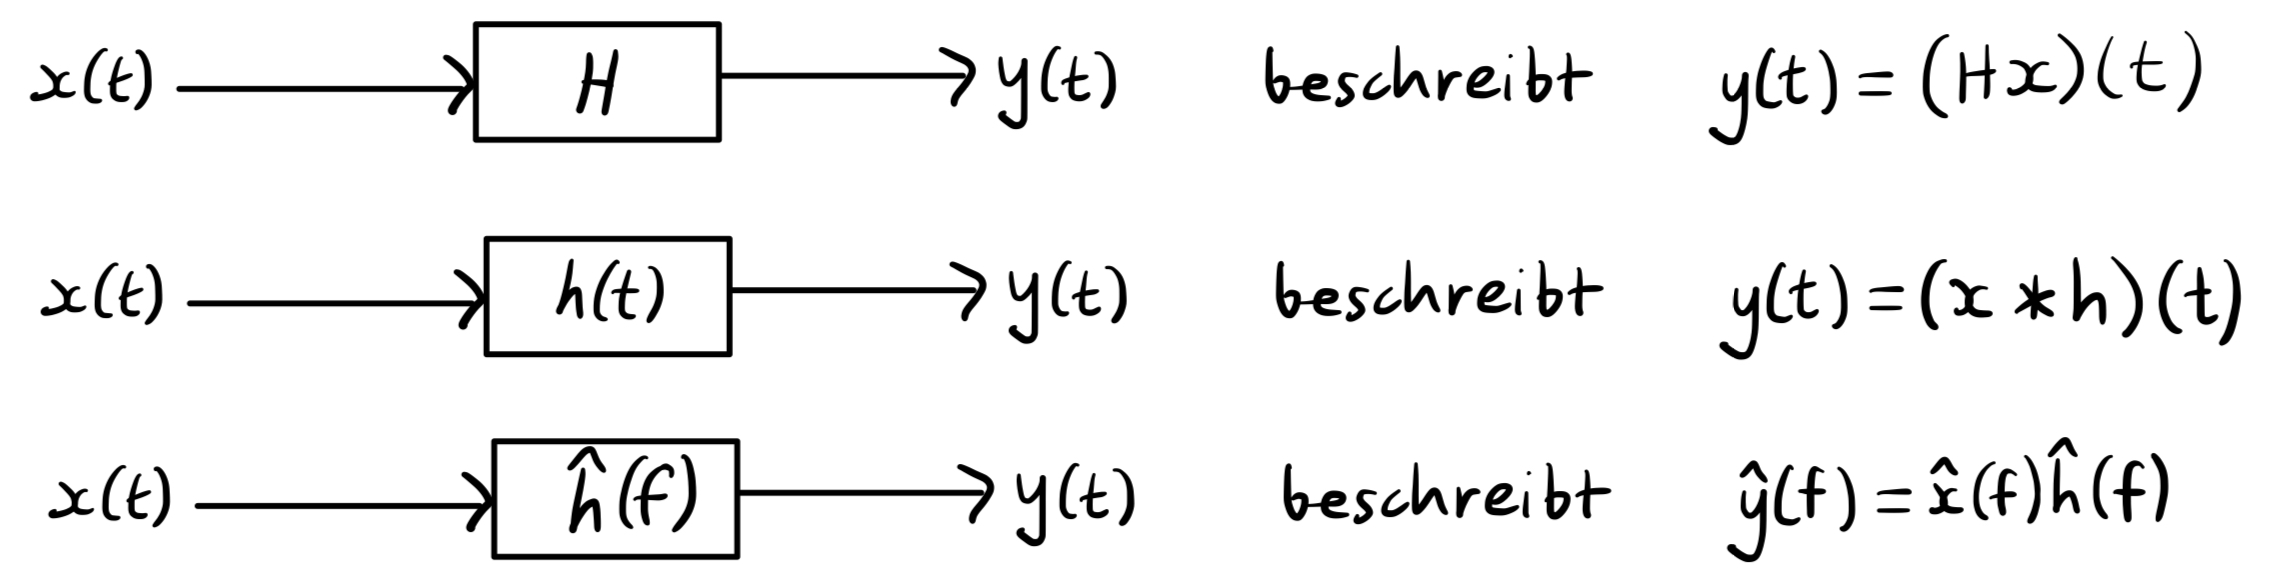
\includegraphics[width=0.9\linewidth]{docimgs/Blockschaltilder.jpg}

\vfill \null
\pagebreak

\section*{Kaskadierung von LTI-Systemen}

\vspace*{-0.5cm}
\begin{itemize}[leftmargin=0pt]
    \item[] Wir betrachten die Kaskadierung von zwei LTI-Systemen $H_1$ und $H_2$. Die Frage ist nun, ob $H_1$ und $H_2$ kommutieren, bzw. ob gilt, dass $H_1H_2 = H_2 H_1$.
    \begin{center}
        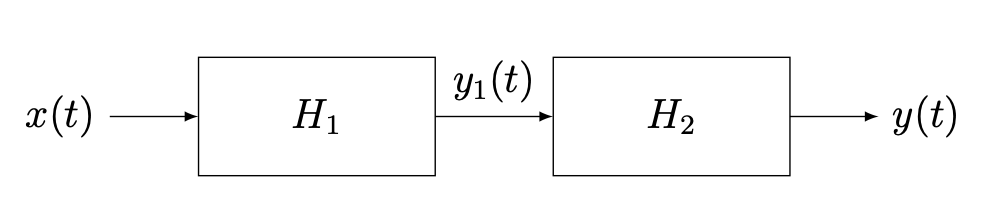
\includegraphics[width=0.7\linewidth]{docimgs/Kaskadierung.png}
    \end{center}
    \item[] \textbf{Antwort}: Ja, \textbf{LTI-Systeme kommutieren!}
    \item[] \textbf{Grund}: (Theorem, das nicht in SST1 behandelt wird):
    \item[] Es seien $A$ und $B$ zwei lineare Operatoren auf einem linearen Raum $V$ ausgestattet mit einem positiv definiten inneren Produkt. (z.B. $A$ und $B$ LTI-Systeme, beliebige Matrizen, etc.) Dann sind die folgenden beiden Aussagen äquivalent: \begin{itemize}
        \item[(i)] $A$ und $B$ besitzen eine gemeinsame Eigenbasis.
        \item[(ii)] $A$ und $B$ kommutieren.
    \end{itemize}
    \item[] Wie wir zuvor gesehen haben, haben LTI-Systeme die komplexen Exponentialfunktionen als gemeinsame Eigenbasis. Somit kommutieren LTI-Systeme.
    \item[] Sidenote: Dieses Theorem ist ausserdem essentiell für Physik 2, wobei man in diesem Fall $\hat{A}$ und $\hat{B}$ als \textit{Hermitian Operators} bezeichnet, die genau dann kommutieren, wenn sie eine gemeinsame Eigenbasis haben. (Dieses Kriterium kann v.a. in Quantum Mechanics sehr hilfreich sein.)
    \item[] Berechnen wir nun konkret die Kaskadierung der beiden LTI-Systeme $H_1$ und $H_2$. Dazu nehmen wir $x(t) = e^{2 \pi i f_0 t}$ (Eigenfunktion) und rechnen:
    \item[] 
\begin{tikzpicture}
    % Define the box size and grid spacing
    \draw[step=0.5cm,gray!50,very thin] (0,0) grid (16.5,5
    ); % (0,0) is bottom-left corner, (10,10) is top-right corner
\end{tikzpicture}
    \item[] \fcolorbox{darkblue}{lightblue}{%
    \parbox{\dimexpr\linewidth-2\fboxsep-2\fboxrule\relax}{
    Die Kaskadierung von LTI-Systemen ist somit wieder ein LTI-System mit $\hat{h}(f) = \hat{h}_1(f) \cdot \hat{h}_2(f)$ d.h. $h(t) = (h_1 \ast h_2)(t)$.
}}%
\end{itemize}

\vfill \null
\pagebreak

\section*{Spezielle Eingangssignale}
\vspace*{-0.5cm}
\subsection*{Allgemeine Schwingungen}
\vspace*{-0.5cm}
Wir betrachten das Eingangssignal $x(t) = \displaystyle e^{st}, \hspace{8pt} s \in \mathbb{C}$,
$ \hspace{8pt} \text{wobei }s = \sigma + i 2 \pi f_0, \hspace{12pt} \mathfrak{Re}(s) = \sigma \begin{cases}
    < 0, \\
    = 0, \\
    > 0,
\end{cases}$
\begin{itemize}[leftmargin = 0pt]
    \item[] dann $x(t) = \textcolor{myblue}{e^{\sigma t}}\textcolor{mygreen}{e^{i 2 \pi f_0 t}}, \hspace{12pt} \mathfrak{Re}(x(t)) = e^{\sigma t}\cos (2\pi f_0 t)$
    \item[] $\textcolor{myblue}{e^{\sigma t}}$ beschreibt die \textcolor{myblue}{Einhüllende} und $\textcolor{mygreen}{e^{i 2 \pi f_0 t}}$ beschreibt die \textcolor{mygreen}{Schwingung}.
    \item[] Der Ausgang eines Systemes mit Impulsantwort $h(t)$ ist dann:
    \item[] $y(t) = (x \ast h)(t) = \displaystyle\int_{-\infty}^{\infty} h(\tau)e^{s(t-\tau)} \text{d}\tau = e^{st} \underbrace{\int_{-\infty}^{\infty} h(\tau) e^{-s\tau} \text{d}\tau}_{=\text{H}(s)}$
    \item[] $\text{H}(s) = \displaystyle\int_{-\infty}^{\infty} h(\tau) e^{-s\tau} \text{d}\tau$ ist die \textbf{Laplace-Transformierte} von $h(t)$.
\end{itemize}

\vspace*{-0.5cm}
\subsection*{Sinusförmiges Eingangssignal}
\vspace*{-0.5cm}
\begin{itemize}[leftmargin=0pt]
    \item[] Wir betrachten das Eingangssignal $x(t) = \cos(2 \pi f_0 t + \varphi_0) = \frac{1}{2} \displaystyle \textcolor{myblue}{e^{i 2 \pi f_0 t}} e^{i \varphi_0} + \frac{1}{2} \displaystyle \textcolor{myblue}{e^{-i 2 \pi f_0 t}} e^{-i \varphi_0}$
    \item[] Die \textcolor{myblue}{blau markierten Signale} sind die Eigenfunktionen. Als Ausgangssignal erhalten wir:
    \item[] $y(t) = (Hx)(t) = \frac{1}{2}\hat{h}(f_0)\displaystyle e^{i 2 \pi f_0 t} e^{i \varphi_0} + \frac{1}{2}\underbrace{\hat{h}(-f_0)}_{=\hat{h}^\ast (f_0)}e^{-i 2 \pi f_0 t} e^{-i \varphi_0}$
    \item[] $\hspace{20pt} = \frac{1}{2}\left(\hat{h}(f_0)e^{i 2 \pi f_0 t} e^{i \varphi_0} + \left(\hat{h}(f_0)e^{i 2 \pi f_0 t} \displaystyle e^{i \varphi_0}\right)^{\ast}\right) = \mathfrak{Re}\left(  \hat{h}(f_0) e^{i 2 \pi f_0 t} e^{i \varphi_0} \right)$
    \item[] $\hspace{20pt} = \textcolor{myred}{|\hat{h}(f_0)|}\cdot \cos\left(\textcolor{mypurple}{2 \pi f_0 t} + \varphi_0 + \textcolor{myorange}{\text{arg}(\hat{h}(f_0))}\right)$, da $\hat{h}(f_0)$ komplexwertig sein kann.
    \item[] Somit ist das Ausgangssignal auf ein sinusförmiges Eingangssignal ein \textcolor{myred}{skalierter} und \textcolor{myorange}{verschobener} Sinus, der mit \textcolor{mypurple}{derselben Frequenz} oszilliert wie das Eingangssignal.
\end{itemize}

\vspace*{-0.5cm}
\subsection*{Einschaltvorgänge}
\vspace*{-0.5cm}
\begin{itemize}[leftmargin=0pt]
    \item[] Wir betrachten das Eingangssignal $x(t) = \displaystyle e^{2 \pi i f_0 t} \sigma(t) \hspace{15pt}$ (Eigenfunktionen aber nur für $t\geq 0$)
    \item[] Der stationäre Zustand des Ausgangssignals ist $y(t) \displaystyle\xrightarrow{t \to \infty} \hat{h}(f_0) e^{2 \pi i f_0 t}$
    \item[] Das heisst unendlich lange nach dem Einschalten hat der Einschaltvorgang keinen Einfluss mehr. Das System befindet sich im eingeschwungenen Zustand (steady state). (Herleitung im Skript s.54)
\end{itemize}

\pagebreak

\subsection*{Fourierreihen}
\vspace*{-0.5cm}
\begin{itemize}[leftmargin=0pt]
    \item[] Was passiert, wenn der Input $x(t)$ ein beliebiges periodisches Signal ist?
    \item[] Aus KomA, Ana2 und NuS2 wissen wir, dass wir jede periodische Funktion als Fourierreihe darstellen können. Wir nehmen also an, dass unser Eingangssignal $x(t)$ $T-$periodisch ist. Dann:
    \item[] \fcolorbox{darkblue}{lightblue}{%
    \parbox{\dimexpr\linewidth-2\fboxsep-2\fboxrule\relax}{
        $$x(t) = x(t + T) = \sum_{k=-\infty}^{\infty} c_k e^{\frac{2 \pi i k t}{T}}, \hspace{12pt} \text{wobei} \hspace{12pt} c_k = \frac{1}{T}\int_0^T x(t) e^{-\frac{2 \pi i k t}{T}} \text{d}t \hspace{12pt} \forall k \in \mathbb{Z}$$
        \hspace{33pt} Gemäss Nr. 21 aus der Formelsammlung wird dieses $x(t)$ fouriertransformiert zu:
        $$(\mathcal{F}x)(f) = \hat{x}(f) = \mathcal{F}\left\{ \sum_{k = -\infty}^{\infty} c_k e^{\frac{2 \pi i k t}{T}}\right\} = \sum_{k = -\infty}^{\infty} c_k \delta\left( f - \frac{k}{T} \right) \hspace{12pt} \forall k \in \mathbb{Z}$$
    }}%
    \item[] \textbf{Eigenschaften der Fourierreihen}\begin{itemize}
        \item[(i)] Fourierreihen existieren nur für periodische Signale.
        \item[(ii)] Periodische Signale haben immer ein "diskretes" Frequenzspektrum.
        \item[(iii)] $c_k$ sind die komplexen Koeffizienten und beschreiben das Signal im Frequenzbereich.
        \item[] Wir schreiben $x(t) = x(t+T) \; \transform{}{1} \; c_k$
        \item[] Die $c_k$ beschreiben die Gewichte des Deltakamms.
        \item[] \begin{center}
            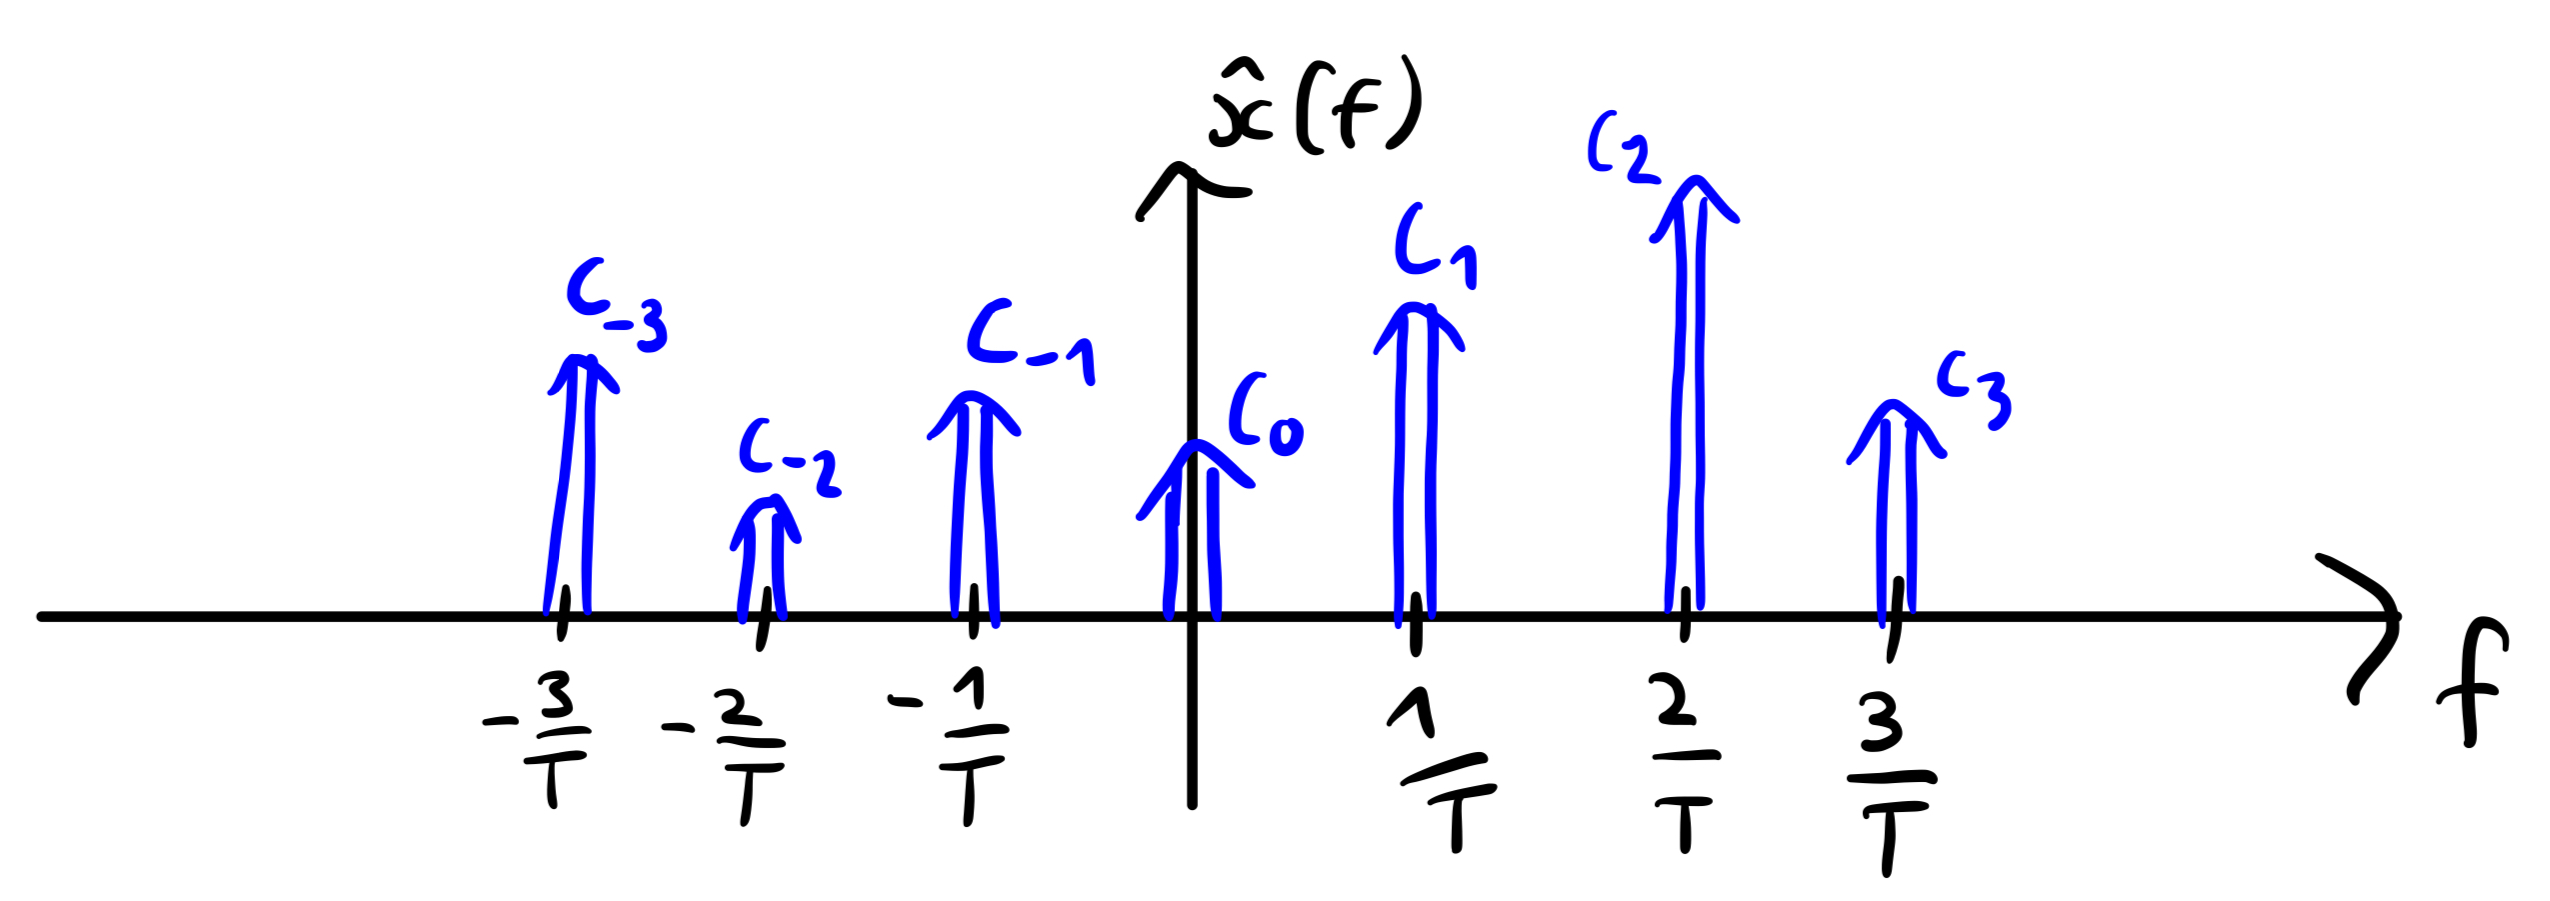
\includegraphics[width=0.55\linewidth]{docimgs/delta_gewichtet.jpg}
        \end{center}
        \item[] Eigentlich ist das Spektrum kontinuierlich, da es für alle Frequenzen definiert ist, es hat jedoch nur an Vielfachen von $1/T$ Komponenten, die ungleich null sind.
        \item[] \begin{center}
            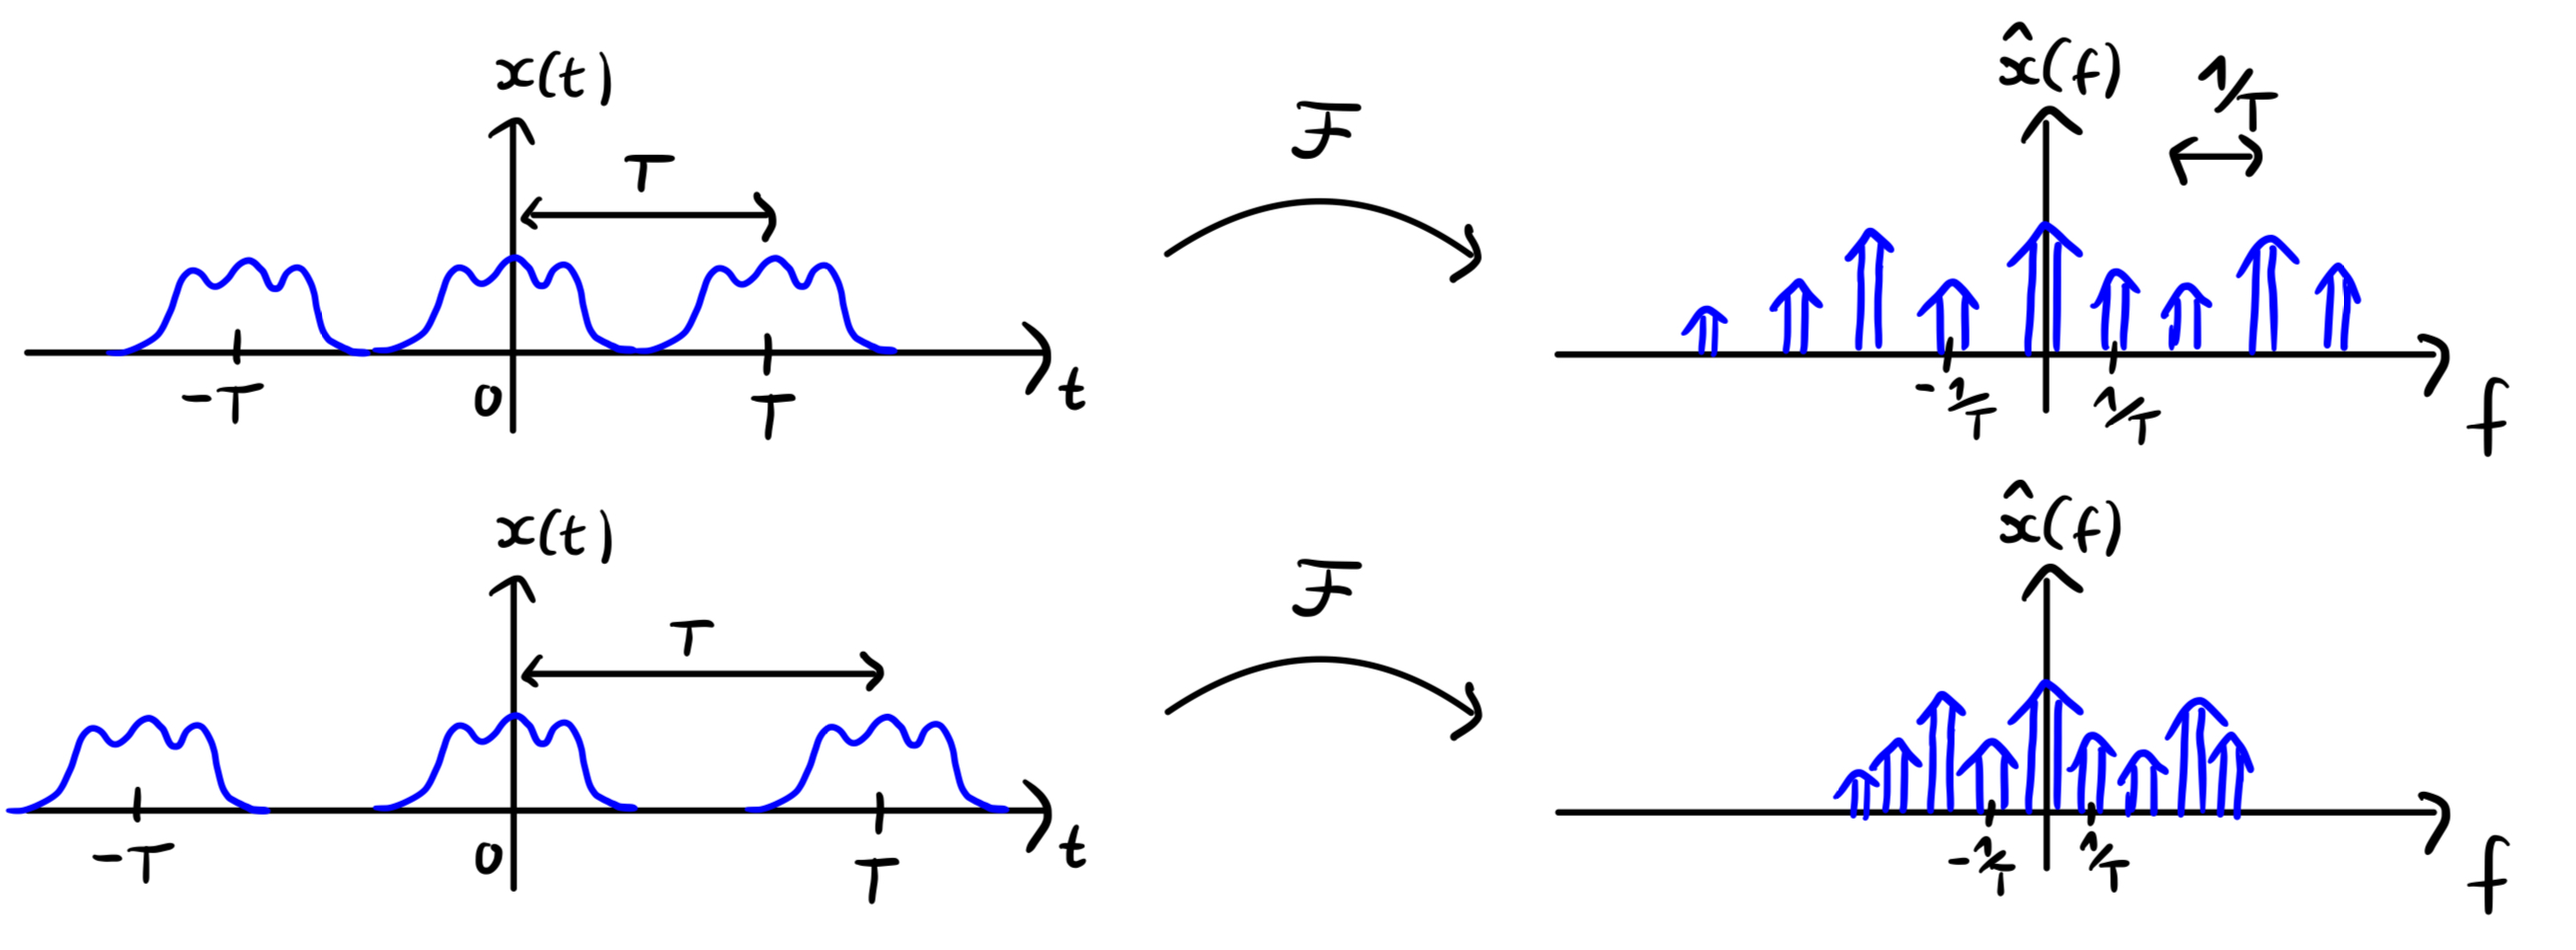
\includegraphics[width=0.8\linewidth]{docimgs/T_increase.jpg}
        \end{center}
        \item[] Wenn $T \to \infty$, dann $1/T \to 0$ und somit wird die Fourierreihe zu einem Integral. Das "diskrete" Spektrum wird kontinuierlich.
    \end{itemize}
     
\end{itemize}

\pagebreak

\subsection*{Periodische Eingangssignale an LTI-Systemen}
\begin{itemize}[leftmargin=0pt]
    \item[] Eingangssignal: $x(t) = \displaystyle\sum_{k = -\infty}^{\infty} c_k e^{\frac{2 \pi i k t}{T}}$
    \item[] Zur Erinnerung: $\left(H \displaystyle e^{2 \pi i f_0 \cdot}\right)(t) = \hat{h}(f_0) e^{2 \pi i f_0 t}$, wobei $e^{2 \pi i f_0 t}$ Eigenfunktionen sind. Hier mit $f_0 = \displaystyle\frac{k}{T}$
    \item[] Dank Linearität und Stetigkeit gilt $\left(H x\right)(t) = \left(H \displaystyle\sum_{k = -\infty}^{\infty} c_k e^{\frac{2 \pi i k \cdot}{T}}\right)(t) = \displaystyle\sum_{k = -\infty}^{\infty} c_k \left(He^{\frac{2 \pi i k \cdot}{T}}\right)(t)$
    \item[] \fcolorbox{darkblue}{lightblue}{%
    \parbox{\dimexpr\linewidth-2\fboxsep-2\fboxrule\relax}{
        $$\hspace{-30pt} \implies y(t) = (Hx)(t) = \sum_{k = -\infty}^{\infty} \smash{\underbrace{c_k \hat{h}\left(\frac{k}{T}\right)}_{d_k}} e^{\frac{2 \pi i k t}{T}}$$
        \vspace*{0.15cm}
    }}%
    \item[] Das Ausgangssignal auf ein $T-$periodisches Eingangssignal ist auch $T-$periodisch.
\end{itemize}

\vspace*{-0.5cm}
\subsection*{Deltakamm}
\vspace*{-0.5cm}
Ein Deltakamm ist die Summe von um $T$ zeitverschobenen Deltafunktionen. (Periode $T$)
$$\delta_T(t) = \sum_{k = -\infty}^{\infty} \delta(t-kT) \hspace{8pt} \transform{51.}{1.5} \hspace{8pt} c_k = \frac{1}{T} \hspace{12pt} \forall k \in \mathbb{Z}$$
Die Antwort eines LTI-Systems auf den Deltakamm $\delta_T(t)$ berechnet sich wie folgt:
$$y(t) \overset{\text{LTI}}{=} (h \ast \delta_T)(t) = \left(h \ast \sum_{k = -\infty}^\infty \delta(\cdot - kT) \right)(t) \overset{\text{LIN}}{=} \sum_{k = -\infty}^\infty \left(h \ast \delta(\cdot - kT)\right)(t) = \sum_{k = -\infty}^\infty h(t-kT),$$
wobei wir in der letzten Umformung verwendet haben, dass die $\delta-$Funktion das Einselement der Faltung ist.

\vspace*{-0.5cm}
\subsection*{Poissonsche Summenformel}
\vspace*{-0.5cm}
\begin{itemize}[leftmargin=0pt]
    \item[] Somit antworten LTI-Systeme auf das Eingangssignal $x(t) = \delta_T(t)$ mit $y(t) = \displaystyle\sum_{k = -\infty}^\infty h(t-kT)$.
    \item[] $y(t)$ ist $T-$periodisch und kann somit als Fourierreihe $\displaystyle\sum_{k = -\infty}^\infty d_k e^{\frac{2 \pi i k t}{T}}$ entwickelt werden.
    \item[] Wegen $x(t) \; \transform{51.}{1} \; \frac{1}{T} \; \forall k \in \mathbb{Z}$  und da gemäss oben $d_k = c_k \hat{h}\left(\frac{k}{T}\right)$ erhalten wir:
    \item[] \fcolorbox{darkblue}{lightblue}{%
    \parbox{\dimexpr\linewidth-2\fboxsep-2\fboxrule\relax}{
        $$\textbf{Poissonsche Summenformel:} \hspace{12pt} \sum_{-\infty}^\infty h(t-kT) = \frac{1}{T} \sum_{-\infty}^\infty \hat{h}\left(\frac{k}{T}\right)e^{\frac{2\pi i k t}{T}}
        $$
    }}%
\end{itemize}



\vfill \null
\pagebreak

\subsection*{Prüfungsaufgabe: Frühjahr 2024, Aufgabe 1.a) ii, iii, iv }

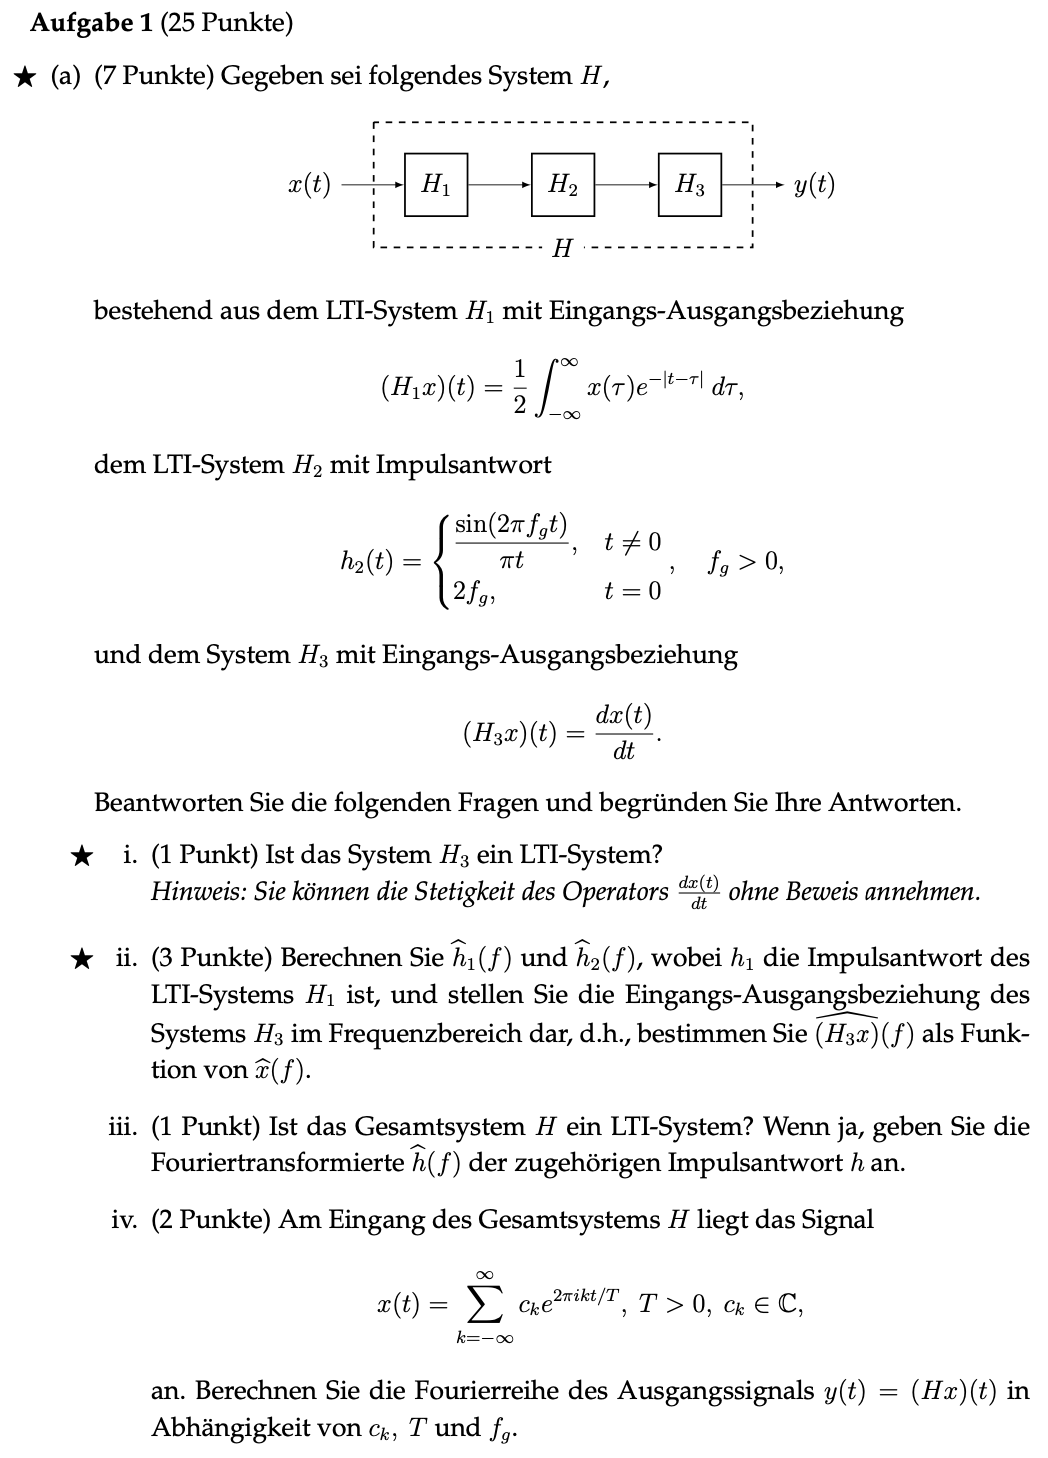
\includegraphics[width=0.85\linewidth]{docimgs/2024_ex1a.png}

\pagebreak


\begin{tikzpicture}
    % Define the box size and grid spacing
    \draw[step=0.5cm,gray!50,very thin] (0,0) grid (16.5,21
    ); % (0,0) is bottom-left corner, (10,10) is top-right corner
\end{tikzpicture}

\pagebreak

\subsection*{Prüfungsaufgabe: Frühjahr 2024, Aufgabe 1.d) i, ii}


\includegraphics[width=0.9\linewidth]{docimgs/2024_ex1d_1.png}\\
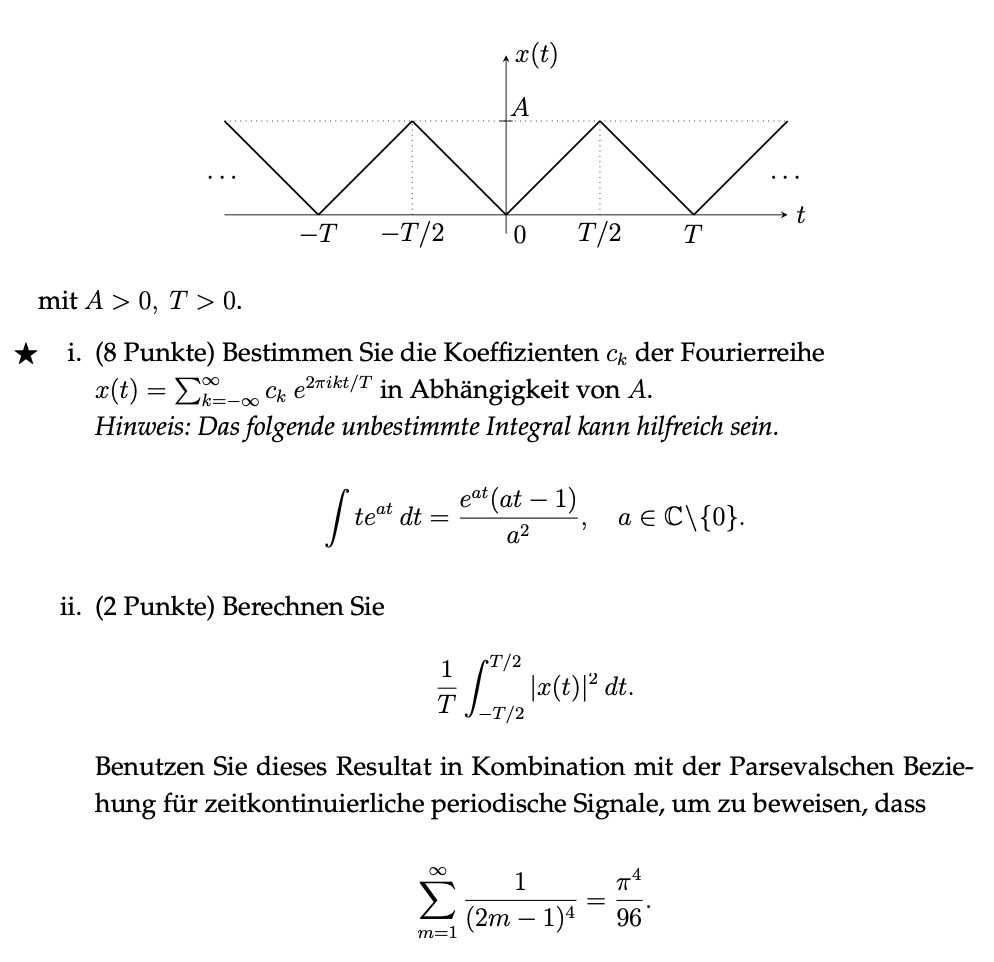
\includegraphics[width=0.9\linewidth]{docimgs/2024_ex1d_2.png}

\vfill \null
\pagebreak


\begin{tikzpicture}
    % Define the box size and grid spacing
    \draw[step=0.5cm,gray!50,very thin] (0,0) grid (16.5,21
    ); % (0,0) is bottom-left corner, (10,10) is top-right corner
\end{tikzpicture}

\end{document}